\documentclass[10pt]{article}
\usepackage[margin=0.8in]{geometry}\usepackage[T1]{fontenc}\usepackage{tikz,url}
\begin{document}\section*{CI tracked-path output handling}
Four Rust jobs failed before compilation because the tracked-path list exceeded the CI helper's 16MiB buffered-stdout limit. This PR's added evidence crosses that boundary.
\begin{center}\begin{tabular}{lr}Input&Bytes\\\hline Pinned base&16,604,789\\Buffered limit&16,777,216\\PR head&17,277,485\end{tabular}\end{center}
\begin{center}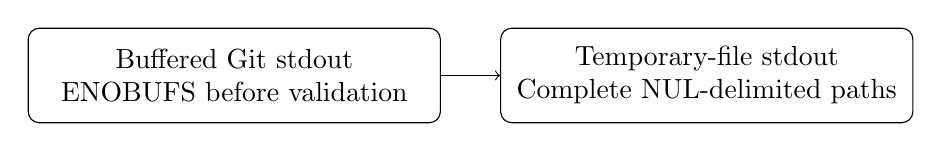
\begin{tikzpicture}[every node/.style={draw,rounded corners,align=center,text width=5cm,minimum height=1.2cm}]
\node (a) at (-3,0) {Buffered Git stdout\\ENOBUFS before validation};
\node (b) at (3,0) {Temporary-file stdout\\Complete NUL-delimited paths};
\draw[->] (a)--(b);
\end{tikzpicture}\end{center}
\subsection*{Correction and controls}
Git stdout is written to a private temporary file and read in full. Classification rules and compiler gates are unchanged. Standard error remains bounded; Git errors still propagate. Temporary files are removed on success and failure.

A real Git index with 80,000 archive paths and two source names exceeds 16MiB, including a source name containing UTF-8 and a newline. The old helper fails this regression with ENOBUFS. The corrected helper passes all 14 scope tests, including sparse inputs, dependency traversal, path handling and failure cleanup.

Read-only source discovery on the actual checkout completed: 2,164 source files and 196 embedded inputs; no checkout materialization. The selected-source path digest is recorded in \texttt{live.stdout}. No performance inference is drawn from test durations. No Rust algorithm or scientific workload changed.
\subsection*{Evidence and limits}
Baseline and corrected native receipts, source hashes, exact path-list byte counts and Node release verification accompany \texttt{status.json}. Complete CI logs remain at the linked GitHub jobs and private hash-bound paths; extracted error lines are included. The first local attempt found no Node on PATH, so no tests ran. The subsequent checks used privately installed Node 22.23.4 matching CI and its official SHA256 manifest.

Sources: repository \texttt{ci-scope.mjs} and its tests; official Node documentation \url{https://nodejs.org/api/child_process.html}. Editable diagram: \texttt{flow.svg}. Remote checks for the corrected revision remain pending publication; local success does not establish remote CI completion.
\end{document}
